%=========================================================================
% (c) 2014, 2015 Josef Lusticky

\section{Spirent configuration}\label{sec:setup-spirent}
Custom iMix, named AMS-IX, was configured according to the AMS-IX statistics described in
subsection~\ref{sub:analysis-metodology-generation}.
Figure~\ref{fig:setup-amsix-imix} shows the configuration window for custom iMix definition
from the Spirent TestCenter Application.
One device was configured on each interface and it was assigned IPv4 and IPv6 addresses, as described in section~\ref{sec:setup-hardware}.
The {\it{Respond to ping}} option was enabled to test the connection.

\begin{figure}
	\centering
	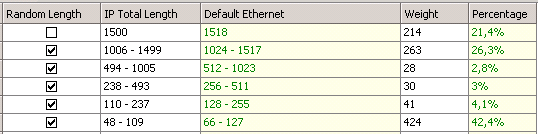
\includegraphics[width=14.5cm,keepaspectratio]{fig/amsix-imix.png}
	\caption{AMS-IX iMix}
	\label{fig:setup-amsix-imix}
\end{figure}

Two traffic patterns were configured for each IP version - one generates a single L4 flow and the other
generates 32 L4 flows.
To test the routing performance of the Linux kernel with full BGP table, 
another traffic pattern was configured.
The pattern uses randomly generated IP destination address for each packet
to avoid having the previous lookup result cached.
All traffic patterns can be configured to generate fixed frame size or custom AMS-IX iMix.
